#MySQL Fabric: 10'
## Fabric - HLA
A python framework for managing, replicating and scaling mysql servers.

  -  aggregate servers in high availability groups
  -  configure single-master replication topologies
  -  monitor and heal failures
  -  director for rw/split
  -  fabric connectors \(caching db topology\)


%http://mysqlmusings.blogspot.it/2013/10/mysql-fabric-high-availability-groups.html


## Fabric - HLA
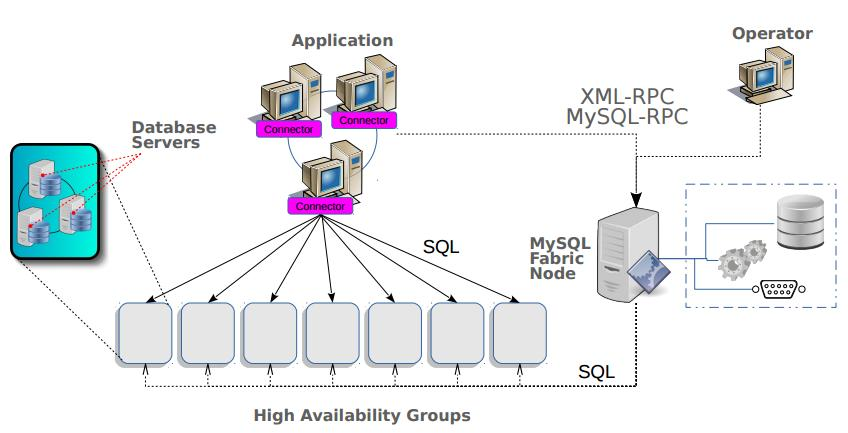
\includegraphics[height=6.6cm,width=12cm]{images/mysql-fabric-hla.jpg}



\column[t]{.5\linewidth}

\end{columns}



\iffalse
Fedora / CentOS / RHEL 7
    ```
    yum -y install \href{https://dev.mysql.com/get/mysql-community-release-el7-5.noarch.rpm}{http://bit.ly/1yhSViu} # MySQL Community repo
    yum -y install mysql-utilites
    ```
\fi



## Setup the lab
Setup and check the course environment.
```
$ docker-compose up -d
$ docker-compose ps
$ docker inspect -f '{{.Name}} {{.NetworkSettings.IPAddress}}'
```

Check the 'fabric' container: we will access all servers from this
 one which includes *all* mysql tools and utilities.
```
$ docker exec -ti fabric_fabric_1 /bin/bash
fabric$
```



## Setup - II
Image with the training infrastructure (fabric, database and docker nodes).
\\
Configure credential in $encrypted$ (mysql\_config\_editor)
 or clear-text (my.cnf) files to avoid wasting time during
the training.
 \\


%## Setup - III
%*empty*
%

## Introducing mysqlfabric
The training covers:

  -  \code{manage [setup|start|ping|stop|teardown]}
  -  group - manage high availability groups
  -  server - manage, clone, provision and decommission servers
  -  provider - manage server providers (eg. openstack, ...)

Further functionalities:

  -  statistics, dump, role, user,
  -  threat, sharding, snapshot, event




## Test Driven Installation
The installation is test-driven via a provided nose script.
Students will be guided in fixing all the tests.
Testing fabric installation (node reachability, user existence, ...)

```
fabric$ cd /code
fabric$ nosetests -v
test_root_access_nodes('m.docker', {'password': 'root', 'user': 'root'}) ... fail
..
test_fabric_access_nodes('m.docker', {'password': 'fabric', 'user': 'fabric'}) ... fail
...
test_fabric ... ERROR
test_fabric_node ... ERROR
```




## Test Driven Installation
Setup fabric server via fabric.cfg . \\
Students will be guided in fixing all the tests.

```
$ mysqlfabric manage setup / start
$ mysqlfabric ping ...
```



 #Replication Groups: 30'
## Create a Group
Create a replication group and adding
servers. \\

Promoting one server as a master. \\
\code{mysqlfabric dump servers}
\\
Adding spare servers. \\

Monitoring failover. \\
```
# mysqlfabric group [create|promote|activate] $GROUP
...
```



##
Import data and check replication status using python tools.

```
mysqldbimport --server=$MASTER ... sakila.sql
mysqldbcompare --server1=$MASTER --server2=$SLAVE \
  --all
```



## Connecting to a group
Configure python clients
\begin{pycode}
from mysql.connector import connect, fabric
c = connect(fabric={host: .., port: .., user: ..},
    autocommit=True,
    database='sample', **sql_user)
c.set_property(mode=fabric.MODE_READWRITE, group="my-cluster-1")
\end{pycode}
\\
Test R/W split and balancing with nose.
```
nosetests -vs test_script.py -m rwsplit
```



 #Troubleshooting: 20'
## Provisioning a new slave
When binlogs have been purged / expired, you need to
import from another server.\\

Caveats on big databases. \\

Provision a new slave with
```
mysqlfabric server clone $GROUP $TARGET
```

Provision a new slave with python utilities
```
# Remove all replica configurations
#  on the slave..
mysql -h$SLAVE -e 'STOP SLAVE;RESET MASTER;'

# ..and reinitialize it
mysqldbcopy --source=$MASTER --destination=$SLAVE
    --rpl-user=fabric:fabric --rpl=master
    --all --drop-first
```



\iffalse
    ## Provisioning a new slave
    Provision a new slave in two steps (eg. large database or requiring tweaks)

      -  check that replica user is provisioned on the master;
      -  create a custom dump.sql;
      -  add --rpl=master;

    \begin{minted}
    cat > data.sql <<EOF
    -- ignore previous changelogs
    -- and trust the backup only
    STOP SLAVE;
    RESET MASTER;

    EOF

    mysqldbexport >> data.sql \
     --server=root:pass@master \
     --rpl-user=repl:rpass \
     --export=master \
     --rpl=master \
     --all

    mysqldbimport --server=root:root@slave \
     data.sql
    \end{minted}

\fi


 #Failover: 20'
## Enabling and Testing Failover
Enabling failover and stopping a master. \\

Checking automatic failover. \\
```
#nosetests -vs --nologcapture fabric-poc.py -m failover &
#mysqladmin shutdown -h $MASTER
```

Re-ingesting a failed master. \\
```
mysqlfabric server set_status  f484d0ed-ecea-11e4-9118-0242ac110039  spare
mysqlfabric server set_status  f484d0ed-ecea-11e4-9118-0242ac110039  secondary
```



 #Provisioning: 20'
## Provisioning new container via docker
Show the provisioning interface (docker, openstack). \\

\begin{pycode}
# mysql.fabric.providers.dockerprovider
class MachineManager(AbstractMachineManager):
    """Manage Docker Containers."""
    def create(self, parameters, wait_spawning):
        ...
    def search(self, generic_filters, meta_filters):
        ...
    def destroy(self, machine_uuid):
        ...
\end{pycode}



## Docker Provisioning

Provisining and deleting containers. \\

Adding provisioned container to ha groups. \\

```
# Register a provider (requires docker in http)
mysqlfabric provider register mydocker \
    user password \
    http://172.17.42.1:2375  \
    --provider_type=DOCKER

# Create new server
mysqlfabric server create mydocker \
    --image=name=mysql-fabric   \
    --flavor=name=v1            \
    --meta=command="mysqld --log-bin=foo"

# List servers
mysqlfabric server list docker
```



## Docker Provisioning
Improving the docker provisioning.

Curious? Vote this training!

```
...
```


\iffalse
## Title
```
#
```

\fi




## Wrap Up

  -  Replication is easier with Fabric and MySQL 5.6
  -  You can clone servers
  -  Failover is just one command ahead
  -  You can't re\-ingest failed masters (luckily;)
  -  Try Fabric with Docker!




## That's all folks!
\begin{center}
Thank you for the attention! \\\\
\insertauthor
\end{center}



\end{document}
